
\documentclass[a4paper,12pt]{article}

\usepackage[utf8]{inputenc}
\usepackage[T1]{fontenc}
\usepackage{graphicx}
\usepackage{float}
\usepackage{geometry}
\usepackage{booktabs}
\usepackage{tikz}

\usetikzlibrary{arrows.meta,positioning}

\geometry{margin=2.5cm}

\setlength{\parindent}{0pt}
\setlength{\parskip}{0.5em}

\title{Bericht}
\author{Jiaqi Wang}
\date{\today}

\begin{document}

\maketitle


\section{Optimierung des ESP32-Codes}

In dieser Woche wurde der ESP32-Code weiter optimiert und das Hindernis am Motor montiert. Anschließende Tests zeigten, dass die Bewegung des Motors und das Verhalten des Hindernisses im erwarteten Bereich lagen.

Zur Vereinfachung der Bedienung wurden die Parameter \textit{Encoder CPR} und \textit{Tolerance} aus der PC-Oberfläche entfernt. Der CPR-Wert wird nun direkt im ESP32-Code festgelegt, da der verwendete EC11-Encoder eine feste Auflösung von $4{,}5^\circ$ pro Count besitzt. Daraus ergibt sich ein fester Wert von 80 Counts pro Umdrehung. Die \textit{Tolerance} bleibt im Code mit einem Standardwert hinterlegt und wird für den normalen Betrieb nicht mehr vom Benutzer eingestellt.

Zusätzlich wurde ein absoluter Winkelgrenzwert eingeführt. Da das montierte Hindernis bei ungefähr $\pm 60^\circ$ den Boden berühren kann, ist der Standardwert des Limits auf $60^\circ$ gesetzt. Dieser Wert kann weiterhin über die PC-Software angepasst werden.

Außerdem wurde ein zusätzlicher IO-Pin des ESP32 mit dem \textit{EN}-Pin des A4988-Treibers verbunden. Wenn die PC-Software den Not-Stopp-Befehl sendet, wird dieser Pin auf High gesetzt. Dadurch wird der A4988-Treiber deaktiviert und der Motor kann sofort gestoppt werden. Auf diese Weise wurde eine softwaregesteuerte Not-Stopp-Funktion umgesetzt.

Für den Neustart des ESP32 wurde zusätzlich die Funktion \texttt{ESP.restart()} verwendet. Damit kann der ESP32 über die PC-Software per Software neu gestartet werden, ohne dass die Stromversorgung manuell getrennt werden muss.



\section{Optimierung der PC-Software}

In dieser Woche wurde auch die PC-Software weiter optimiert. Dabei wurde eine modulare Benutzeroberfläche umgesetzt, sodass die einzelnen Funktionsbereiche klar voneinander getrennt sind. Dadurch kann die Anwendung auch dann intuitiv bedient werden, wenn der Benutzer die genaue Funktion der App noch nicht kennt.

Die Oberfläche besteht nun aus fünf Hauptmodulen: \textit{WiFi}, \textit{Status Log}, \textit{Parameter}, \textit{LED Control} und \textit{Motor Control}. Jedes Modul enthält nur die Funktionen, die zu seinem jeweiligen Aufgabenbereich gehören. Dadurch wird die Bedienung übersichtlicher und die Fehlerwahrscheinlichkeit bei der Nutzung reduziert.


\begin{figure}[h]
    \centering
    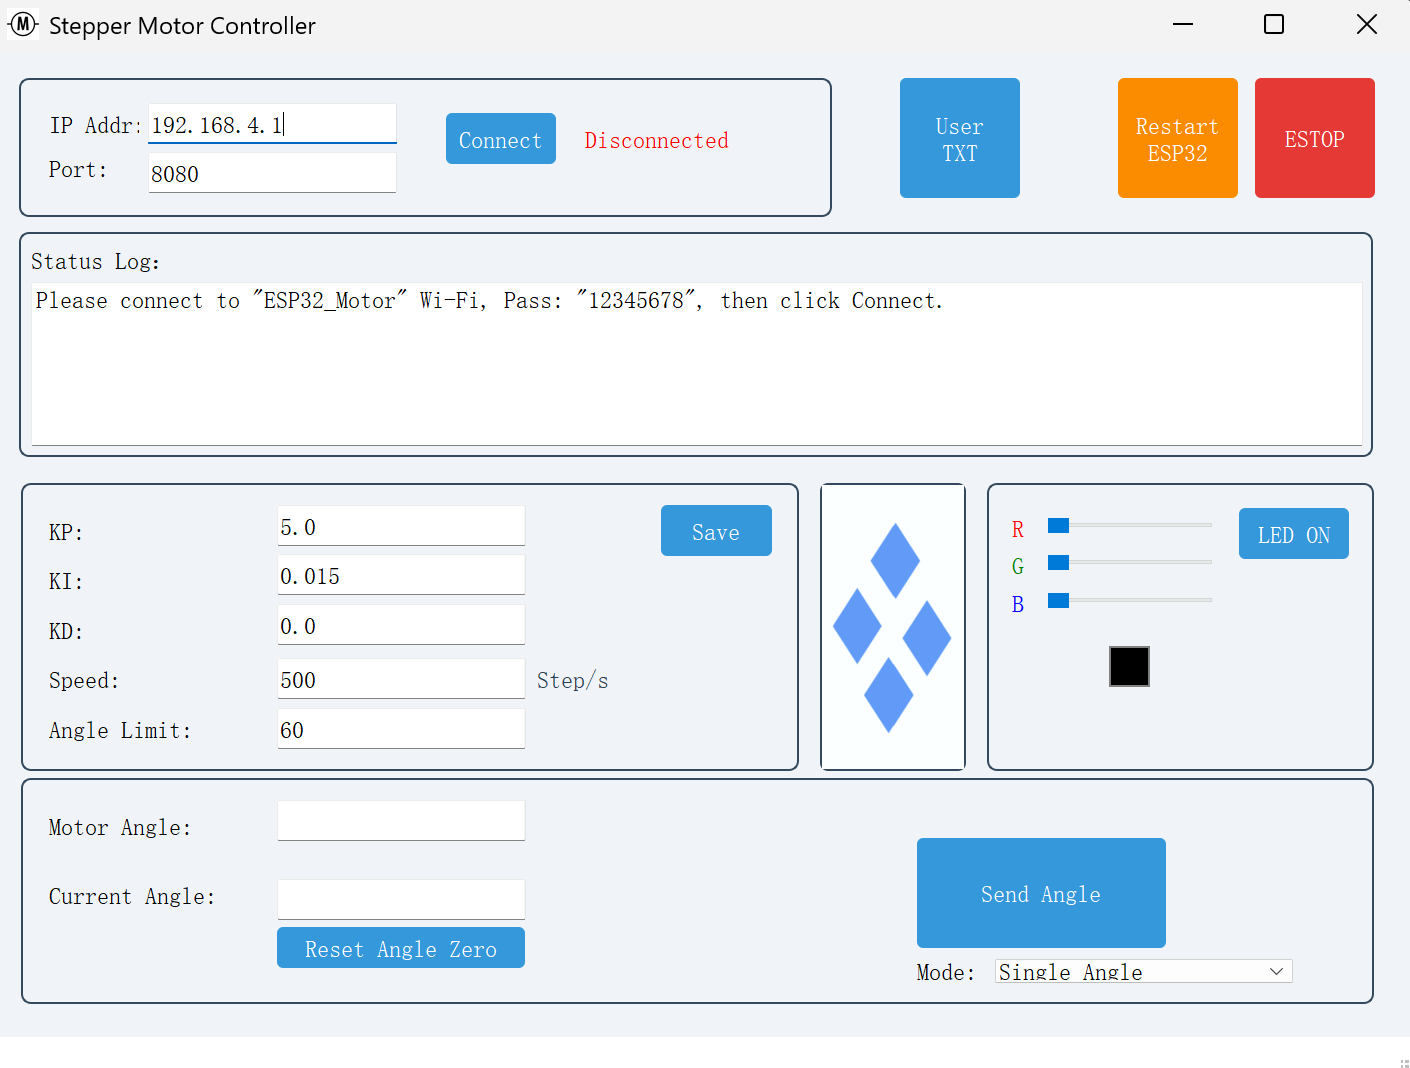
\includegraphics[width=0.8\textwidth]{ui.png}
    \caption{Modulare Benutzeroberfläche der PC-Software}
    \label{fig:pc_software_ui}
\end{figure}


Zusätzlich wurde das Farbschema der Schaltflächen vereinheitlicht. Innerhalb der Module werden die normalen Bedienknöpfe in Blau dargestellt. Globale oder sicherheitsrelevante Funktionen befinden sich oben rechts in der Anwendung. Der \textit{ESTOP}-Button ist rot markiert, da er für den Not-Stopp des Motors verwendet wird. Der Button zum Neustart des ESP32 ist orange dargestellt. Zusätzlich gibt es einen \textit{User TXT}-Button, über den eine Bedienungsanleitung für die App geöffnet werden kann.



\section{To-do-Liste}

Als nächster Schritt sollen weitere Tests mit dem EC11-Encoder durchgeführt werden. Da der Encoder eine Auflösung von $4{,}5^\circ$ pro Count besitzt, kann es im Betrieb häufig zu Abweichungen von etwa $4{,}5^\circ$ bis $9^\circ$ kommen. Deshalb soll durch zusätzliche Messungen analysiert werden, ob diese Genauigkeit für die Anwendung ausreichend ist.

Außerdem soll ein optischer Sensor integriert werden. Dieser soll eine absolute Winkelreferenz ermöglichen und langfristig die bisherige Speicherung der Position im Flash ersetzen. Dadurch kann die Referenzposition nach dem Einschalten zuverlässiger erkannt und eine automatische Nullstellung umgesetzt werden.

Ein weiterer geplanter Arbeitspunkt ist das feste Verlöten der Schaltung. Dadurch soll der bisherige Versuchsaufbau stabiler und zuverlässiger werden.

Zusätzlich soll die Motor-Control-App auf einem weiteren Ubuntu-Computer installiert und getestet werden, um die Nutzbarkeit der Software auf einem zweiten System zu überprüfen.



\end{document}
